\chapter{\texorpdfstring{\glsdesc{MMLT}}{MMLT}}\label{cha:mmlt}
During lunch, Greg thought about the different types of triangles
Mrs. Minerva had told him about (\cref{cha:triangulations}) and which ones
he liked the most. On one hand he liked triangles with long edges,
on the other hand Greg was very interested in NP-complete problems.
Therefore he decided to find out more about \gls{MMLT}, which forces
the shortest edge to be as long as possible and was proven 
NP-complete \cite{mmlt_complexity}.

\begin{problem}[\gls{MMLT}]
  \hfill
  \begin{labeling}{\hspace{4em}}
    \item[\textbf{Given:}]
      Set of points in the plane \(P\) and implicitly their induced segments
      \(S_P\) (see \cref{def:induced_segments})
    \item[\textbf{Sought:}]
      Triangulation \(\gls{Topt}\subseteq S_P\) of \(P\) which maximizes
      \(\min\limits_{s\in \gls{Topt}} |s|\) 
      with \(|s|\) being the length of the segment \(s\)
  \end{labeling}
\end{problem}

When playing around with some small instances \footnote{Greg drew them
on napkins in the cafeteria.}, Greg discovered two 
properties of \gls{MMLT}[s]. An optimal solution need not be unique as
\cref{fig:non_unique_optimal} shows. Additionally 
\cref{fig:nonoptimal_flips} is an example where an edge flip
\todo{explain edge flips} is necessary in a local optimum to gain 
global optimality. Therefore it is not always possible to retrieve an
optimal \gls{MMLT} solution by starting with an arbitrary
triangulation and applying locally optimal edge flips.

\begin{figure}[ht]
  \centering
  \includegraphics[width=0.5\textwidth]{img/non_unique_optimal.jpg}
  \todo[inline]{replace}
  \caption{Example of different optimal solutions for the same point set.\label{fig:non_unique_optimal}}
\end{figure}

\begin{figure}[ht]
  \centering
  \includegraphics[width=0.5\textwidth]{img/example_nonoptimal_flips.jpg}
  \todo[inline]{replace}
  \caption{Example of necessary locally non-optimal flips.\label{fig:nonoptimal_flips}}
\end{figure}

\begin{definition}[Edge Length Order]
  Given a set of edges \(E\) representing a set of line segments
  \(S\) and two edges \(e_{s_i}, e_{s_j} \in E\) representing two
  line segments \(s_i,s_j \in S\), respectively. Let \(|s|\) for
  \(s \in S\) be the segment length and \( s_i < s_j \) the
  lexicographical order of \(s_i, s_j \in S\). The edge length
  order is defined as  
  \[
    e_{s_i} < e_{s_j}
    \iff |s_i| < |s_j|
    \lor ((|s_i| = |s_j|) \land (s_i < s_j)).
  \]
\end{definition}

\begin{definition}[Edge Length Index]
  Given a set of edges \(E\) representing a set of line segments
  \(S\) and an edge \(e \in E\). The edge length index \(|e|\) is the
  index of \(e\) in \(E\) sorted by edge length order.
\end{definition}

\begin{problem}[\gls{MMELIT}]
  \hfill
  \begin{labeling}{\hspace{4em}}
    \item[\textbf{Given:}]
      Set of points in the plane \(P\)
    \item[\textbf{Sought:}]
      Topological triangulation \(\gls{Topt} = (V,E)\) of \(P\)
      which maximizes the minimum edge length index: 
      \(\min\limits_{e\in E} |e|\).
  \end{labeling}
\end{problem}

\begin{theorem}
  The optimal edge in a \gls{MMELIT} solution is unique.
\end{theorem}

\begin{proof}
  \ldots\todo[inline]{proof}
\end{proof}

\begin{theorem}
  Every optimal \gls{MMELIT} solution is an optimal \gls{MMLT} solution.
\end{theorem}

\begin{proof}
  \ldots\todo[inline]{proof}
\end{proof}

\begin{verbatim}
  IP:
  - maximize min. edge index
  - no conflicting edges
  - for every edge: either edge or crossing edge picked
  - n^2 variables, O(n^4) restrictions
\end{verbatim}
\todo[inline]{notes}

\section{Separators}
He tried to identify the good, the bad, and the ugly edges. Bad are
clearly all short edges as they can worsen the \gls{MMLT} solution.
Step by step, Greg found the set of all segments which were
shorter than a certain threshold and named them the
``short segments''.

\begin{definition}[Short Edges]\label{def:short_edges}
  Given a set of edges \(E\) representing a set of line segments
  \(S\). Short edges within \(E\) are all edges with an edge
  length index smaller than a certain threshold:
  \[
    \gls{Eshort}[(P, \ell)] := \{ e \in E : |e| < \ell \}
  \]
\end{definition}

The next observation Greg made is that there were some long segments
which cross the short segments. Greg called them ``separators'' as
they separate the endpoints of short segments. When the shortest
segment which is part of the \gls{MMLT} solution has separators, it
can (under certain conditions) be replaced by a longer segment to
improve the solution. Therefore separators are the good segments.

\begin{definition}[Separators]\label{def:separators}
  Given a set of edges \(E\) representing a set of line segments
  \(S\) and a set of conflicts \(C \subseteq E^2\). The set of separators
  \(\gls{Esep}[(E, C, e)]\) for an edge \(e \in E\) are all edges
  that improve the \gls{MMELIT} solution, i.e. all in \(C\) with
  \(e\) \gls{conf} edges which have a higher edge length index:
  \[
	  \gls{Esep}[(E,C,e)] := \{
		  \gls{esep} \in E:
		  |e| < |\gls{esep}|\land \{e,\gls{esep}\} \in C
	  \}
  \]
\end{definition}

Finally, there are the ugly segments which are short but have no
separators such that they can not be replaced \footnote{\ldots which
is not their fault!}. A special case are segments which do not cross
at all --- for example those on the convex hull. The ugliest segment
is the shortest of all ugly segments \gls{enose}.

\begin{definition}[Shortest Non-separable Edge]
  Given a set of edges \(E\) representing a set of line segments
  \(S\) and a set of conflicts \(C \subseteq E^2\). The
  \emph{shortest non-separable edge} \gls{enose} is the edge with 
  the smallest edge length index which has no separators:
  \[ 
    \gls{enose} := \argmin\limits_{
      e \in E :
      \gls{Esep}[(E,C,e)] = \emptyset
    } |e|
  \]
\end{definition}

Greg pities the ugly segments because nobody likes them even though
they are not bad. So he tries to find something where they are good
at. When the boy thinks back to the art class, he remembers that a 
triangulation \(T\subseteq S_P\) of a point set \(P\) is a maximum
set of non-crossing segments (\cref{def:triangulation_subdivision}).
So any segment \(s \in S_P\) that is
not crossed by another segment \(\gls{scross} \in T\) has to be part
of \(T\) itself. A similar property applies to the ugly segments
in a \gls{MMELIT}: Every segment \(s \in S_P\) with no separators
is either part of an optimal \gls{MMELIT} solution \gls{Topt} or
crosses a shorter (or equal length) segment
\(\gls{scross} \in \gls{Topt}\).

\begin{theorem}[upper bound]\label{thm:upper_bound}
  Given a set of edges \(E\) representing a set of line segments
  \(S\) and a set of conflicts \(C \subseteq E^2\). Let
  \gls{Topt} be an optimal \gls{MMELIT} solution for \(P\). Every
  segment \(s\) without separators is an upper bound for \gls{Topt}:
  \[
    \forall s \in S_P,~ \gls{Esep}[(P,s)] = \emptyset :
    \min\limits_{s_{\min} \in \gls{Topt}} |s_{\min}| \leq |s|
  \]
  which is equivalent to
  \[
    \forall s \in S_P:~ \lnot\exists \gls{Esep} \in S_P :
    |s| < |\gls{Esep}| \land~ s, \gls{Esep}~ \gls{cross}
    \implies \min\limits_{s_{\min} \in \gls{Topt}} |s_{\min}| \leq |s|
  \]
\end{theorem}
%---------------------------------------------------------------------##########
\begin{proof}
  Assume
  \[
    \exists s \in S_P,~ \gls{Esep}[(P,s)] = \emptyset :
    \min\limits_{s_{\min} \in \gls{Topt}} |s_{\min}| > |s|.
  \]
  This implies \(s \not\in \gls{Topt}\) and
  \[
    \forall s' \in S_P :
    |s'| \leq |s| \implies s' \not\in \gls{Topt}.
  \]
  With \(\gls{Esep}[(P,s)] = \emptyset\) it follows that
  \[
    \forall \gls{scross} \in S_P :
    s, \gls{scross}~\gls{cross}
    \implies \gls{scross} \not\in \gls{Topt}.
  \]
  This means that for \gls{Topt} to be a triangulation \(s\) has 
  to be in \gls{Topt}---which is a contradiction.
\end{proof}

Unfortunately, Greg soon found an example where the ugly segments did
not help: \cref{fig:upper_bound_tightness}. In this instance, there
are short segments which have conflicting (crossing) separators. This
forces one short segment to be part of the optimal triangulation as
only one of the separators can be selected. Therefore the upper bound
for an optimal \gls{MMLT} solution in \cref{thm:upper_bound} is not
tight.

\begin{figure}[ht]
  \centering
  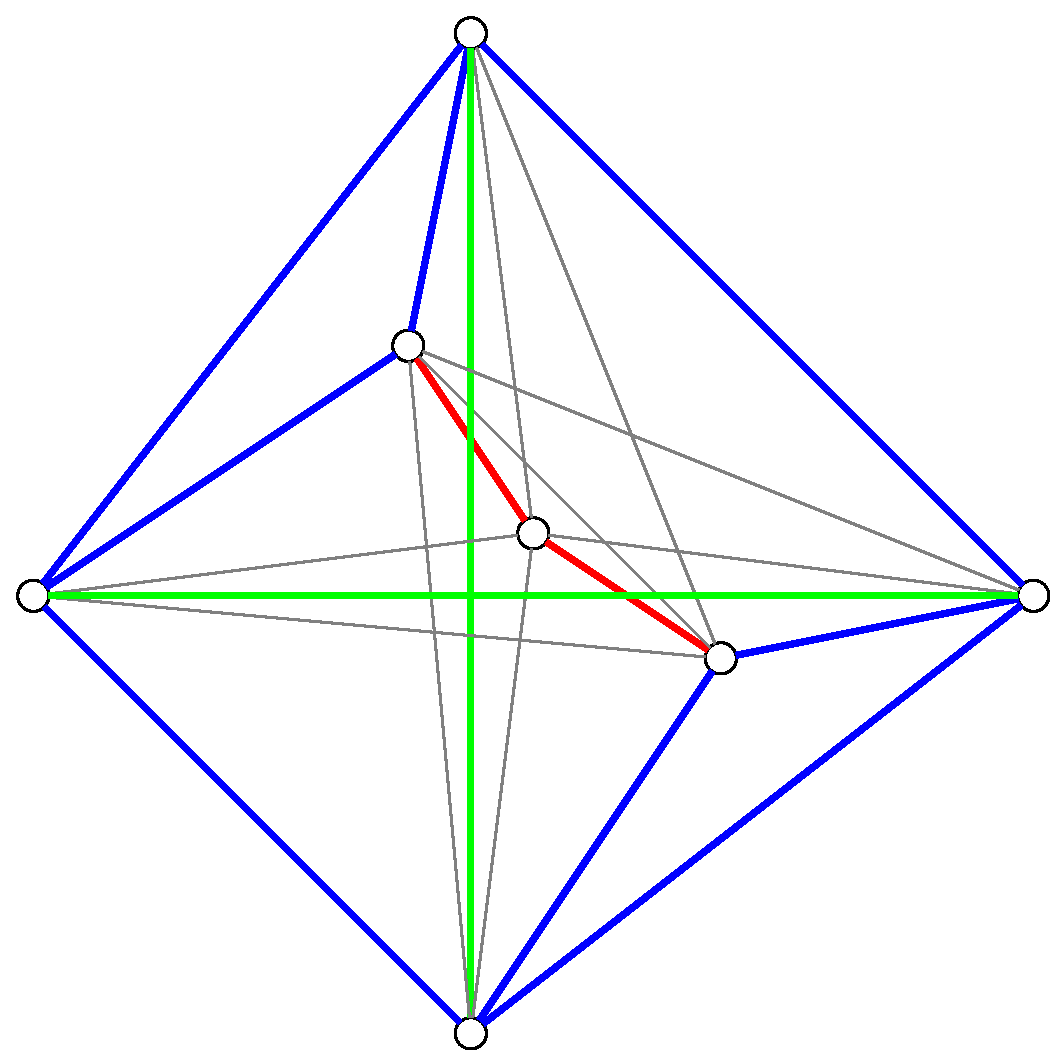
\includegraphics[width=0.5\textwidth]{img/upper_bound_tightness.jpg}
  \todo[inline]{replace}
  \caption{
    \label{fig:upper_bound_tightness}
    Example where the upper bound from \cref{thm:upper_bound} is not 
    tight. One of the short segments (red) is part of an optimal 
    \gls{MMLT} solution because their separators (green) cross. Thus
    the shortest segment in the solution is shorter than the shortest
    one of all segments without separators (blue).
  }
\end{figure}  

Greg remembered that he had met conflicting segments in 
\cref{fig:nonoptimal_flips} already. By conflicting he meant that the
separator \gls{Esep} of a segment \(s\) either crossed any segment
\gls{scross} shorter than \(s\) or the separator which replaced
\gls{scross}. 

\begin{definition}[Conflicting Segments]\label{def:conflicting_segments}
  Given planar point set \(P\) and its induced segments \(S_P\). The
  (potentially) conflicting segments for a segment \(s \in S_P\) are:
  \[
    \gls{Sconf}[(P,s)] :=
      \bigcup_{\gls{scross} \in \gls{Eshort}[(|s|)]}
      \gls{scross} \cup \gls{Esep}[(\gls{scross})]
  \]
\end{definition}

Greg immediately started to rethink his earlier understanding of ugly
segment. His opinion was that short segments with only conflicting
separators were as ugly as those with no separators at all. The latter
ones are even a special case of the first group. So he changed
\cref{thm:upper_bound} to take conflicting separators into account. A 
segment may be part of an optimal \gls{MMLT} solution because all of
its separators interfere with other segments. The following
\namecref{thm:tight_upper_bound}
assumes knowledge of the optimal triangulation, so conflicting segments 
can only be found iteratively after the triangulation has already be 
calculated for shorter segments. However, we will see how conflicts can 
be formulated independently later on.

\begin{theorem}[tight upper bound]\label{thm:tight_upper_bound}
  Given a point set \(P\) and its induced segments \(S_P\). Let
  \gls{Topt} be an optimal \gls{MMLT} solution for \(P\).
  Every segment \(s\) without non-conflicting separators is an upper
  bound for \gls{Topt}:
  \[
    \gls{Esep}['(P,s)] := 
    \{
      \gls{Esep} \in \gls{Esep}[(P,s)] : 
      \gls{Esep} \cup (\gls{Topt} \cap \gls{Sconf}[(P,s)])~\gls{ncross}
    \}
  \]
  \[
    \forall s \in S_P : \gls{Esep}['(P,s)] = \emptyset \implies
    \min\limits_{s_{\min} \in \gls{Topt}} |s_{\min}| \leq |s|
  \]
  \todo[inline]{can we get \gls{Topt} out of the bound?}
\end{theorem}


\begin{proof}
  This proof is very similar to the proof of \cref{thm:upper_bound}.
  Assume
  \[
    \exists s \in S_P :
    \gls{Esep}['(P,s)] = \emptyset
    \land \min\limits_{s_{\min} \in \gls{Topt}} |s_{\min}| > |s|.
  \]
  That implies \(s \not\in \gls{Topt}\) and
  \[
    \forall s' \in S_P : |s'| \leq |s| \implies s' \not\in \gls{Topt}.
  \]
  
  If \(\gls{Esep}[(P,s)] = \emptyset\) itself, according to
  \cref{thm:upper_bound} it holds that
  \[ \min\limits_{s_{\min} \in \gls{Topt}} |s_{\min}| \leq |s|\]
  which is a contradiction.
  
  Now assume \(\gls{Esep}[(P,s)] \not= \emptyset\). The
  following holds:
  \[
    \forall \gls{Esep} \in \gls{Esep}[(P,s)] :
    \gls{Esep} \cup (\gls{Topt} \cap \gls{Sconf}[(P,s)])~\gls{cross}.
  \]
  
  With \gls{Topt} being a triangulation this implies
  \[
    \forall \gls{Esep} \in \gls{Esep}[(P,s)] :
    \gls{Esep} \not\in \gls{Topt}.
  \]
  Therefore
  \[
    \forall s_c \in S_P,~ s, s_c~\gls{cross} : 
    s_c \not\in \gls{Topt}.
  \]
  That means that \(s\) has to be in \gls{Topt} -- which is a
  contradiction.
\end{proof}

\begin{theorem}[tightness]\label{thm:tighness}
  The bound of \cref{thm:tight_upper_bound} is tight. That is, let
  \(T\) be a feasible \gls{MMLT} solution and
  \(s_{\min} = \argmin\limits_{s \in T} |s|\) with no
  non-conflicting separators:
  \[
    \lnot\exists
    \gls{Esep} \in \gls{Esep}[(s_{\min})] : 
    \gls{Esep} \cup (\gls{Topt} \cap \gls{Sconf}[(s_{\min})])~\gls{ncross}
  \]
  
  Then \(T\) is optimal.
\end{theorem}

\begin{proof}
  \ \todo[inline]{Assume not optimal, compare optimal, prove not optimal}
\end{proof}

\section{Set Cover}

As a consequence of \cref{thm:tight_upper_bound} with 
\cref{thm:tighness}, we introduce the following smaller (in terms
of input and output size) problem \gls{NCS}.
For \(S = \{s \in S_P : |s| \leq |\gls{enose}|\}\) an optimal 
solution \gls{Sopt} for \gls{NCS} has the same shortest segment 
as an optimal \gls{MMLT} solution \gls{Topt}:
\[
  \min\limits_{s \in \gls{Sopt}} |s|
  = \min\limits_{s \in \gls{Topt}} |s|
\]

\begin{problem}[\gls{NCS}]
  \hfill
  \begin{labeling}{\hspace{4em}}
    \item[\textbf{Given:}]
      Set of short segments \(S\) and their separators \gls{Esep}.
    \item[\textbf{Sought:}]
      Set of \gls{ncross} segments \(\gls{Sopt} \subseteq S \cup
      \bigcup\limits_{s \in S} \gls{Esep}[(s)] \) which contains
      for each segment \(s \in S\) either the segment itself or at
      least one separator \(\gls{Esep} \in \gls{Esep}[(s)]\) and
      maximizes \(\min\limits_{s \in \gls{Sopt}} |s|\).
  \end{labeling}
\end{problem}

The \gls{NCS} problem can be modeled as a weighted set cover problem. 
Therefore it is also NP-hard.

\begin{verbatim}
  IP:
  - maximize min. edge index
  - no conflicting edges
  - for every short edge: either edge or separator picked
  - worst case: n^2 variables, O(n^4) restrictions
  - random points: O(n) variables, < O(n^3) restrictions?
\end{verbatim}
\todo[inline]{notes}

\begin{problem}
  \hfill
  \begin{labeling}{\hspace{4em}}
    \item[\textbf{Given:}]
      Set of short segments \(S\) and their separators \gls{Esep}.  
    \item[\textbf{Sought:}]
      \todo[inline]{here comes the reduction}
  \end{labeling}
\end{problem}

\section{Algorithm}
Now that Greg knew all about \gls{MMLT} he could start developing
\cref{alg:mmlt}. It consists of three main components: Constructing
the partial intersection graph, running a binary search over the short
segments and solving the smaller \gls{NCS} problem in each step, and
using the resulting segments in a constrained triangulation.

\todo[inline]{mention segment index and introduce notation \protect\ensuremath{S_P[i]}}
\begin{algorithm}
  \DontPrintSemicolon
  \KwIn{Planar point set \(P\)}
  \KwOut{An optimal \gls{MMLT}} solution for \(P\)
  
  \SetKwData{last}{last}
  \SetKwData{lb}{lb}
  \SetKwData{mid}{mid}
  \SetKwData{ub}{ub}
  
  Generate the induced segments \(S_P\) for \(P\) \;
  Find the shortest non-separable segment \gls{enose}
  and calculate intersections for 
  \(\gls{Eshort}[(|\gls{enose}|)]\) and their separators \;
  Set the lower bound \(\lb = 0\) \;
  Set the upper bound \ub such that \(S_P[\ub] = \gls{enose}\) \;
  Set \(\last = \emptyset\) \;
  \While{\lb < \ub}{
    Set \(\mid = \left\lceil\frac{\lb + \ub}{2}\right\rceil\) \;
    Find optimal \gls{NCS} solution \gls{Sopt}
    for \(\gls{Eshort}[(P,|S_P[\ub]|)]\) \linebreak
    without using any segment from \(\gls{Eshort}[(P,|S_P[\mid]|)]\) \;
    \eIf{there is a solution \gls{Sopt}}{
      Set \(\last = \gls{Sopt}\) \;
      Maximize \lb such that \(|S_P[\lb]| = \min\limits_{s \in \gls{Sopt}} |s|\) \;
      \If{\lb > \ub}{
        \lb = \ub \;
      }
    }{
      \eIf{\(\lb < \mid\)}{
        Set \(\ub = \mid - 1\) \;
      }{
        Set \(\ub = \lb\) \;
      }
    }
  }
  \KwRet{constrained triangulation \gls{Topt} with \last as constraints}
  \caption{\label{alg:mmlt}\gls{MMLT} algorithm}
\end{algorithm}

\section{Intersection Graph}\label{sec:mmlt_intersection_graph}
For a point set \(P\) with \(n\) points in the plane 
the induced segments (see
\cref{def:induced_segments}) have \(\Theta(n^4)\) intersections.
\cite{quadrilaterals_bound} Thus calculating the intersection graph
takes \(\Omega(n^4)\) time.

\begin{verbatim}
  - link to sweep line algorithm
  - sweep line takes O(n^4 \log n) time => brute force is faster
  - adjacency list, because sparse (experiment? proof?)
\end{verbatim}
\todo[inline]{notes}

\begin{algorithm}
  \DontPrintSemicolon
  
  \KwIn{Set of segments \(S\)}
  \KwOut{Intersection graph \(G=(S,C)\) where \(C \subseteq S^2\) 
    are the intersections}
  
  Set \(C = \emptyset\) \;
  \ForEach{\(s \in S\)}{
    \ForEach{\(\gls{scross} \in S\) with \(|s| \leq |\gls{scross}|\)}{
      \If{\(s\) and \gls{scross} are \gls{cross}}{
        Add \(\{s, \gls{scross}\}\) to \(C\) \;
      }
    }
  }
  \KwRet{\(G=(S,C)\)}
  \caption{intersection algorithm}
\end{algorithm}
  
%---------------------------------------------------------------------##########
